\documentclass[dutch]{deltares_manual_style}

\svnid{$Id: ds_um.tex 1 2015-10-01 12:00:00Z rodriqu_dd $}

\usepackage{booktabs}
\usepackage {color}
\definecolor {gray}     {rgb} { 0.4, 0.4, 0.4 }
\definecolor {darkblue} {rgb} { 0.0, 0.0, 0.6 }
\definecolor {cyan}     {rgb} { 0.0, 0.6, 0.6 }
\definecolor {orange}   {rgb} { 1.0, 0.5, 0.0 }
\definecolor {brown}    {rgb} { 0.6, 0.3, 0}
\usepackage {listings}

\lstdefinelanguage {XML} {
    escapechar=\%,
    identifierstyle=\color{brown},
    stringstyle=\color{blue},
    morestring=[b]",
    morecomment=[s]{<?}{?>},
    morecomment=[s][\color{green}]{<!--}{-->},
    keywordstyle=\color{red},
    morekeywords={
        designation,
        icaoCode,
        ilsFreq,
        ilsID,
        name,
        partition,
        pathname,
        range,
        schemaLocation,
        state,
        tora,
        towerFreq,
        trueBRG,
        type,
        units,
        value,
        version,
        xmlns,
        xsi
        } % list your attributes here
    }

\lstset {
    language=XML,
    basicstyle=\ttfamily\footnotesize,
    columns=fullflexible,
    showstringspaces=false,
    commentstyle=\color{gray}\upshape
    }

\graphicspath{{../common/}}

\newcommand{\menuarrow}{$\rightarrow$\xspace}
%\newcommand{\deltashell}{\textrm{Delta Shell}\xspace} % for headings where \, is not allowed

\newenvironment{litemize}{\begin{itemize}\raggedleft}{\end{itemize}}
\newcolumntype{L}{>{\raggedright\arraybackslash}X}
\newcolumntype{C}{>{\centering\arraybackslash}X}
\newcolumntype{R}{>{\raggedleft\arraybackslash}X}
%------------------------------------------------------------------------------
\hypersetup
{
    pdfauthor   = {Deltares},
    pdftitle    = {Wettelijk Toets Instrumentarium (WTI) Handleiding},
    pdfkeywords = {Deltares User Manual},
    pdfcreator  = {LaTeX hyperref},
    pdfproducer = {ps2pdf}
}
%------------------------------------------------------------------------------
%
\renewcommand\BackgroundPicChapter{
    \put(0,0){
    \parbox[b][\paperheight]{\paperwidth}{%
        \vspace{4\baselineskip}
        \hspace{220mm}
        
\includegraphics[width=15mm]{cover/chapter-ribbon.jpg}%
        \vfill
        }
    }
}

%------------------------------------------------------------------------------
%
\begin{document}

\pagestyle{empty}
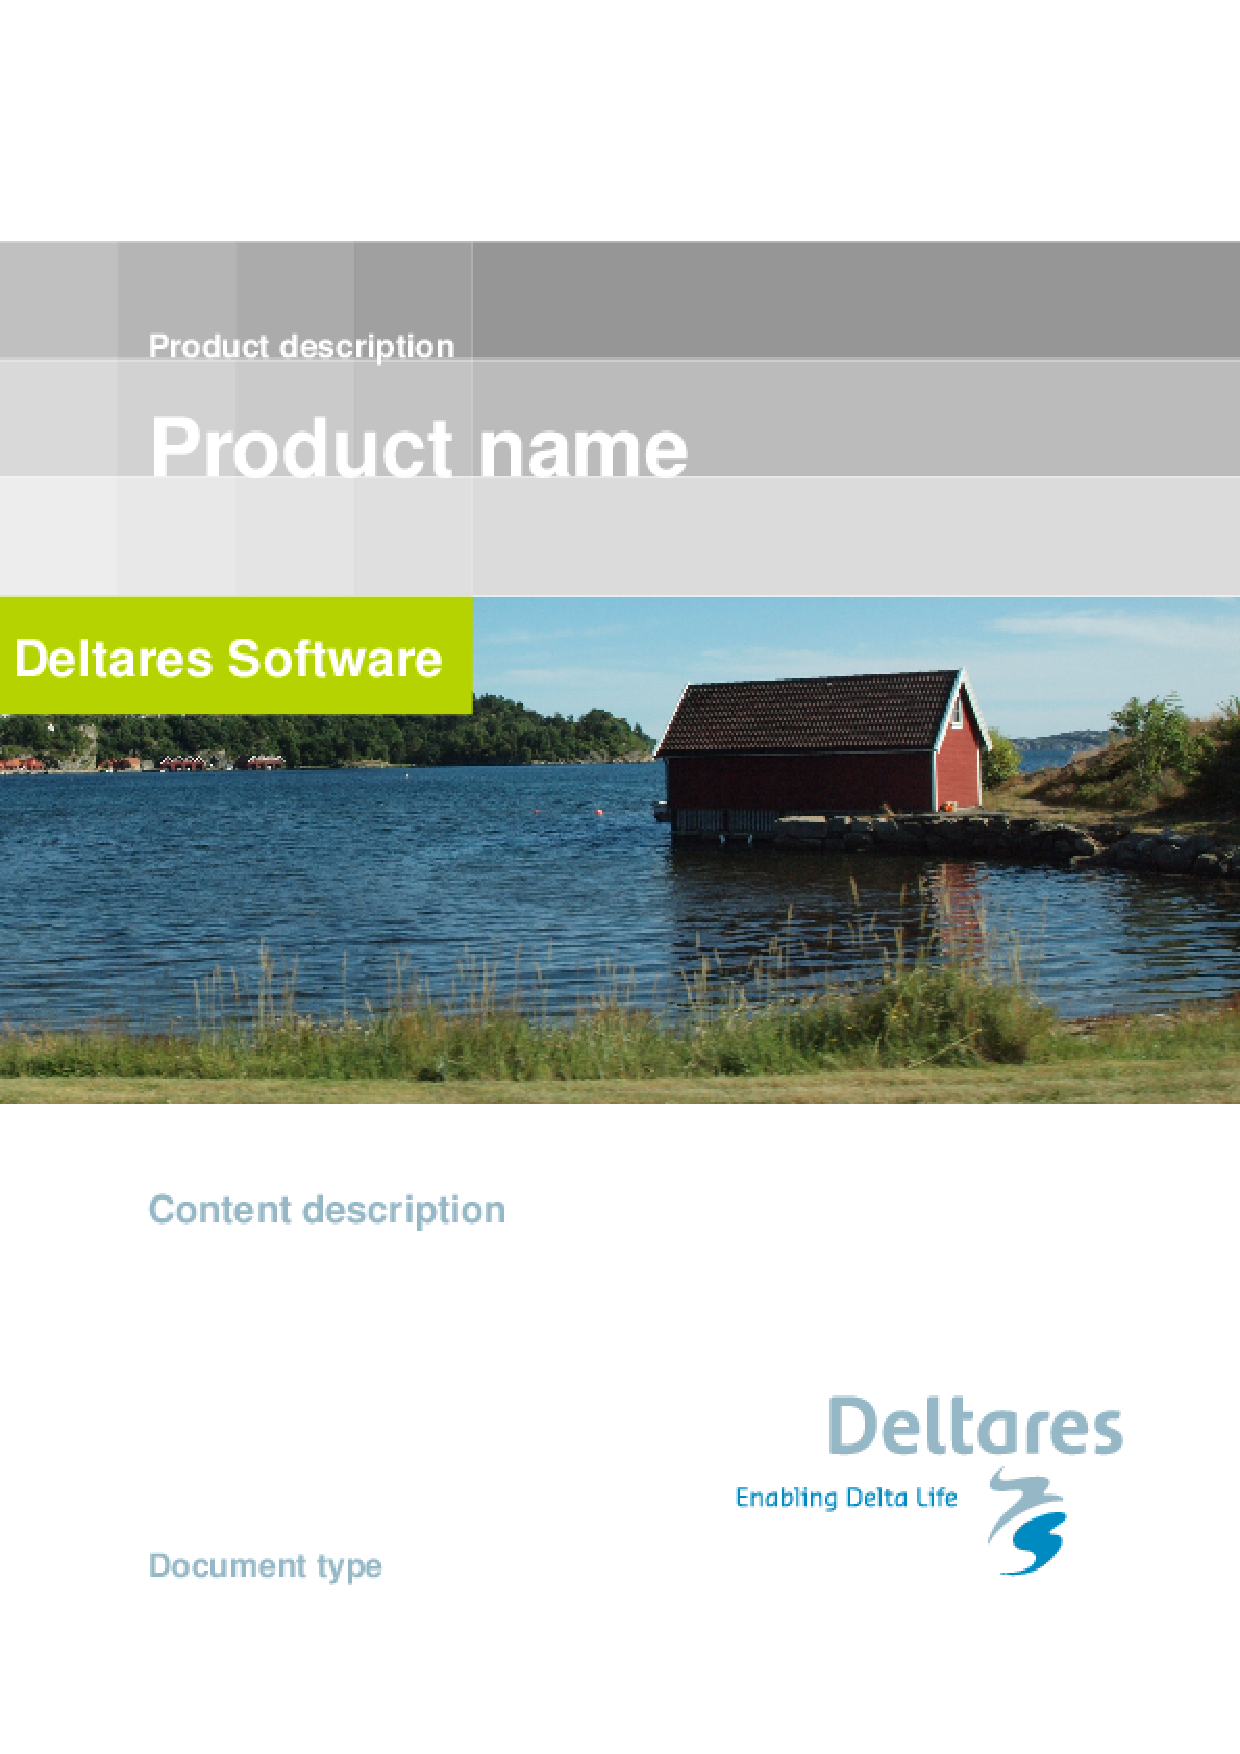
\includepdf[pages=1,offset=72 -70]{cover/default-cover-pages.pdf} % links-rechts past precies
\cleardoublepage

\title{Wettelijk Toets Instrumentarium (WTI)}
\subtitle{}
\manualtype{Gebruikershandleiding}
\version{1.0}
\date{1 november 2015}
\manualtitle

\svnid{$Id: ds_guide.tex 1 2015-08-30 15:39:28Z rodriqu_dd $}

\chapter{Introductie\label{chap:guide}}

\section{Inleiding}
Deze handleiding betreft de Wettelijk Toetsingsinstrumentarium (WTI).

\section{Overzicht}
Om de toegankelijkheid van deze handleiding te bevorderen, wordt er een overzicht van alle onderdelen ge\"{i}ntroduceerd.

\Autoref{chap:ds_overview}: \nameref{chap:ds_overview}, gives a brief introduction to all GUI-components, which are shared between fail mechanisms based on the framework.

\section{Versie informatie}
Productinformatie is op te vragen via Menu | Info. Via de Support organisatie kan het versienummer
vergeleken worden met de vigerende versie. De productinformatie heeft de support
organisatie ook nodig om te controleren welke modules er in de gebruikte Ringtoets versie
zijn geïnstalleerd en u van de juiste ondersteuning te voorzien. De productinformatie geeft
tevens toegang tot de gebruiksvoorwaarden (disclaimer) van het product.

\section{Typographical conventions}
Throughout this manual, the following conventions help you to distinguish between different
elements of text.
\svnid{$Id: typographical_conventions.tex 1 2015-08-30 15:39:28Z mooiman $}  

\begin{longtable*}{|p{2.0in}|p{\textwidth-2.0in-24pt}|} \hline \nobreak
\textbf{Example} & \textbf{Description} \STRUT \\[1ex] \nopagebreak \hline \endhead

\window{Piping} \STRUT \newline \window{Scenarios} &
Title of a window or sub-window.\newline
Sub-windows are displayed in the \window{Module} window and cannot be moved.\newline
Windows can be moved independently from the \window{Module} window, such as the \window{Visualisation Area} window. \\ [1ex] \hline

\menu{Save} \STRUT &
Item from a menu, title of a push button or name of a user interface input field.\newline
Upon selecting this item (click or, in some cases, double click with the left mouse button on it) a related action will be executed; in most cases it will result in displaying some other (sub-)window.\newline
In case of an input field, you are supposed to enter input data of the required format and in the required domain. \\ [1ex] \hline

\STRUT \dir{\textbackslash tutorial\textbackslash DR10\textbackslash asfalt} \newline \file{revetments.csv.mdw} &
Directory names, filenames, and path names are expressed between angle brackets, $<>$. \\ [1ex] \hline

\ginput{27 08 1999} \STRUT &
Data to be typed by you into the input fields are displayed between double quotes.\newline Selections of menu items, option boxes etc.\ are described as such: for instance `select \menu{Save} and go to the next window'. \\ [1ex] \hline

\command{wti-menu} \STRUT &
Commands to be typed by you are given in the font Courier New, 10 points. \\ [1ex] \hline


\includegraphics[height=4mm]{pictures/action_arrow.pdf} \STRUT &
User actions are indicated with this arrow. \\ [1ex] \hline

\unitbrackets{\meter\per\second} \unitbrackets{-} \STRUT &
Units are given between square brackets when used next to the formulae. Leaving them out might result in misinterpretation. \\ [1ex] \hline

\end{longtable*}

\section{Changes with respect to previous versions}
This is the first edition.
\svnid{$Id: ds_guide.tex 1 2015-08-30 15:39:28Z rodriqu_dd $}

\chapter{Installatie\label{chap:install}}

\section{Inleiding}
Deze sectie beschrijft de installatie procedure van de applicatie Ringtoets. Hiervoor is in ieder geval het installatie bestand (Ringtoets Setup*.msi) nodig. Daarnaast worden er enkele eisen aan het besturingssysteem gesteld (zie \Autoref{sec:sysrequirements}). 

\section{Systeemeisen}
\label{sec:sysrequirements}
Voor een goed functioneren van WTI is het wenselijk (of in sommige gevallen nodig) om een computer te hebben die minimaal voldoet aan de volgende eisen:
\begin{itemize}
	\item Microsoft Windows 7 hoger
	\item Microsoft .NET Framework versie 4.0 of hoger
	\item Minimaal een Intel Pentium III/800 MHz processor (of vergelijkbaar)
	\item Minimaal 256(???) MB RAM (1 GB RAM aanbevolen)
	\item Minimale beeldscherm resolutie van 1024x768 pixels
\end{itemize}




\section{WTI installeren en opstarten}
\label{sec:wtiinstall}
De installatie procedure wordt opgestart door op de snelkoppeling dubbel te klikken. Op bijna elke stap kan de procedure voortgezet worden door te drukken op \textit{Volgende}. De eerdere stap van de procedure kan bereikt worden door te klikken op \textit{Vorige}. Door op \textit{Annuleren} te klikken, kan de installatie onderbroken worden. 

Er zijn drie type installaties:
\begin{itemize}
	\item \textbf{Standaard}: de meest gebruikte onderdelen van het programma worden ge\"installeerd. Het programma wordt ge\"installeerd in de map
		
		\dir{C:\textbackslash Program Files (x86)\textbackslash Deltares\textbackslash Wettelijk Toets Instrumentarium (\color[rgb]{0.75,0.75,0.75}versienummer\color[rgb]{0,0,0})}.
		
		Dit is de aanbevolen optie voor de meeste gebruikers.
	\item \textbf{Aangepast}: de te installeren onderdelen en de map waarin het programma zal ge\"installeerd worden, kunnen geselecteerd worden. Door deze optie te kiezen, kan het ook gecontroleerd worden hoe veel ruimte de installatie in beslag zal nemen, en hoe veel ruimte beschikbaar is in de beschikbare volumes.
	\item \textbf{Volledig}: alle onderdelen van het programma worden ge\"installeerd. Het programma wordt ge\"installeerd in de map
		
		\dir{C:\textbackslash Program Files (x86)\textbackslash Deltares\textbackslash Wettelijk Toets Instrumentarium (\color[rgb]{0.75,0.75,0.75}versienummer\color[rgb]{0,0,0})}.
\end{itemize}

Op het moment dat de de installatietype gekozen is, wordt deze daadwerkelijk uitgevoerd door op \textit{Installeren} te klikken. De voortgang van de installatie wordt aangegeven totdat hij klaar is. Op dat moment wordt de installatie procedure volledig afgerond door op \textit{Voltooien}  te klikken.


Als het installatiebestand opgestart wordt nadat het programma ge\"installeerd is, kan de installatie aangepast worden. De mogelijke aanpassingen zijn:
\begin{itemize}
	\item \textbf{Wijzigen}: hiermee kan men opnieuw aangegeven worden welke onderdelen van het programma ge\"installeerd zullen zijn. 
	\item \textbf{Herstellen}: deze optie herstelt de ontbrekende of beschadigde bestanden, snelkoppelingen en registervermeldingen van de huidige installatie.
	\item \textbf{Verwijderen}: de installatie van het Wettelijk Toets Instrumentarium wordt volledig verwijderd van de computer door deze optie te kiezen.
\end{itemize}

Na installatie (\Autoref{sec:wtiinstall}) kan Ringtoets worden opgestart via het startmenu (onder de map Deltares) of door op het bijbehorende icoontje (\Fref{fig:fig2.1}) op het bureaublad dubbel te klikken. 


\begin{figure} [H]
	\centering
		
\includegraphics{figures/chapter_installation/wti_desktop_icon}
	\caption{Ringtoets snelkoppelingsicoon op het bureaublad.}
	\label{fig:fig2.1}
\end{figure}

Er wordt ook een snelkoppeling aangemaakt in het startmenu van Windows. Deze is te vinden in Startmenu $\,\to\,$ Alle programma's $\,\to\,$ Deltares $\,\to\,$ Ringtoets $\,\to\,$ Ringtoets:


\begin{figure} [H]
	\centering
		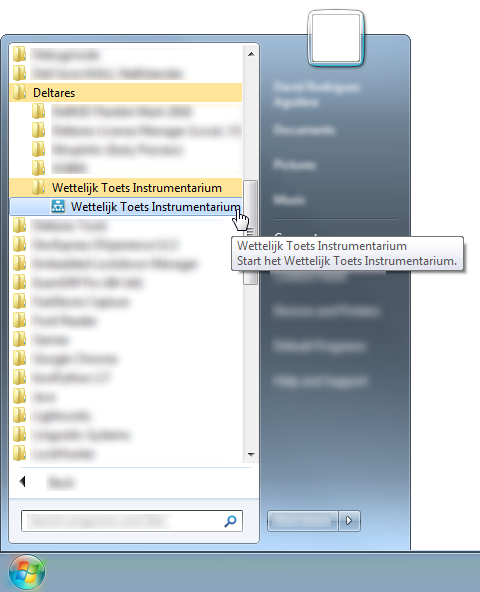
\includegraphics{figures/chapter_installation/rtInAllPrograms}
	\caption{Ringtoets in de startmenustructuur van Windows \color[rgb]{1,0,0} \textbf{Needs to be updated!!!}\color[rgb]{0,0,0}.}
	\label{fig:fig2.2}
\end{figure}


Kort nadat het programma ge\"instaleersd is, is deze snelkoppeling direct te vinden onder het startmenu:


\begin{figure} [H]
	\centering
		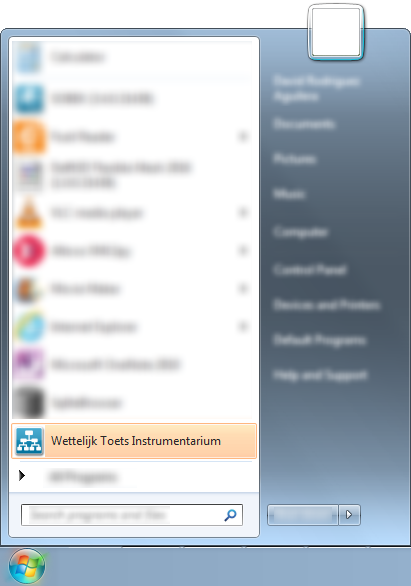
\includegraphics{figures/chapter_installation/rtDirectlyinStartMenu}
	\caption{Ringtoets direct in het startmenu van Windows \color[rgb]{1,0,0} \textbf{Needs to be updated!!!}\color[rgb]{0,0,0}.}
	\label{fig:fig2.3}
\end{figure}














\svnid{$Id: MorphAn_man_Algemeen.tex 41593 2015-08-30 15:39:28Z mooiman $}

\chapter{Projecten, schermen en schermindeling}
	\label{ch:DeltaShell}

In dit hoofdstuk wordt een overzicht gegeven van de algemene functionaliteit van MorphAn. Na een korte introductie wordt in dit hoofdstuk allereerst aandacht besteed aan de projectstructuur die door MorphAn wordt gebruikt. Vervolgens worden de hoofdfuncties van de gebruikersinterface uitgelegd voor alle type beschikbare vensters. Als laatste wordt aandacht besteed aan de mogelijkheden tot importeren en exporteren van data en resultaten.

\section{Project structuur}
	\label{sec:DS_Project_Structure}
MorphAn werkt met een projectstructuur die weergegeven wordt in het \textbf{Project} toolvenster (zie paragraaf \ref{sec:DS_Project_Explorer}). Data en modellen kunnen aan het project worden toegevoegd op de volgende manieren:

\begin{enumerate}
	\item Klik op \textbf{New Folder}, \textbf{New Item} of \textbf{New Model} in de \textbf{Home} tab bovenaan het scherm, zoals weergegeven in figuur \ref{fig:DS_Add_Object}.
	\item Rechtsklik in het \textbf{Project} toolvenster op de gewenste locatie en klik dan op \textbf{New Item...} of \textbf{New Folder}, zoals weergegeven in figuur \ref{fig:DS_Add_Object_Project_Explorer}.
\end{enumerate}

\begin{figure}[H]
	\centering
		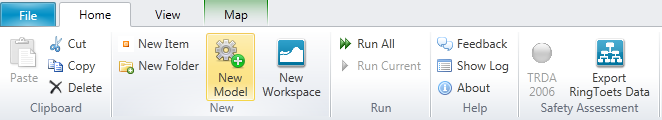
\includegraphics[width=1.0\textwidth]{pictures/Hoofdstuk_Delta_Shell/Home_Ribbon_Add_New_Model.png}
		\caption{Voorbeeld van de Home tab met daarin onder het kopje Add de mogelijkheid tot het toevoegen van een object aan het project.}
	\label{fig:DS_Add_Object}
\end{figure}
\begin{figure}[H]
	\centering
		\includegraphics{pictures/Hoofdstuk_Delta_Shell/DS_Add_Object_Project_Explorer.png}
		\caption{Voorbeeld van het context menu dat naar voren komt bij rechts klikken op het project. Door op Add te klikken krijgt de gebruiker de mogelijkheid objecten aan het project toe te voegen.}
	\label{fig:DS_Add_Object_Project_Explorer}
\end{figure}

De objecten in een MorphAn project zijn doorgaans afgeleid van een van de drie soorten zoals hieronder weergegeven (en nader omschreven):
\begin{itemize}
\item \textbf{Item} - Geeft data weer van een willekeurig type
\item \textbf{Model} - Geeft een model weer
\item \textbf{Folder} - Geeft een folder weer vergelijkbaar met een directory in het windows besturingssysteem
\end{itemize}

\subsection{Item}
Een item kan willekeurige informatie bevatten. MorphAn kent drie type items die altijd aanwezig zijn:
\begin{itemize}
\item Map (World) - Voegt een lege kaart toe aan het project
\item Text Document - Voegt een leeg tekst document toe aan het project
\item Web link - Voegt een weblink toe aan het project
\item MorphAn workspace - Voegt een morphan workspace toe (zie ook paragraaf \ref{ch:Data:MorphAnWorkspace})
\end{itemize}
Naast een item is er doorgaans ook een (document) venster beschikbaar om de inhoud van het item te bekijken en zo mogelijk aan te passen. In dat geval is het venster te openen door dubbel te klikken op het desbetreffende item in het \textbf{Project} toolvenster of via een klik met de rechter muisknop op het item in het project toolvenster en dan op \textit{Open}.

\subsection{Model}
Een model is een rekenkern met bijbehorende invoer en uitvoer. Standaard heeft een model in DeltaShell dus ook een folder \textit{Input} en een folder \textit{Output}. In de input en output folders is er plaats voor items die de invoer en uitvoer beschrijven. Het laten rekenen van een model kan op verschillende manieren:
\begin{itemize}
\item Rechtsklik op het model in het \textbf{Project} toolvenster en dan klik op \textbf{Run Model}
\item Klik op 
\includegraphics{pictures/Hoofdstuk_AandeSlag_nieuw/Run_Arrow.png} (run) of 
\includegraphics{pictures/Hoofdstuk_AandeSlag_nieuw/RunAll_Arrow.png} (run All) in de \textbf{Home} tab van de ribbon (zie ook paragraaf \ref{sec:DS_Toolbar})
\item Selecteer een model en druk op F9, of druk op Ctrl+F9 om alle modellen in het project te laten rekenen
\end{itemize}
Binnen MorphAn is het alleen mogelijk om een model toe te voegen aan een workspace. MorphAn biedt geen modellen aan die buiten een workspace kunnen worden toegevoegd (met uitzondering van de optionele XBeach 1D plugin, zie ook hoofdstuk \ref{ch:Extra:Installation:Options}).

\subsection{Folder}
Een Folder in een MorphAn project is vergelijkbaar met een map, folder of directory in het windows bestandssysteem. Een map kan worden gebruikt om gegevens (items en modellen) te ordenen en groeperen. Folders worden ook gebruikt in Modellen om input items en output items te groeperen.

\section{Interface onderdelen}
	\label{sec:DS:InterfaceOnderdelen}
Figuur \ref{fig:1_MA_Welcome_Page} geeft een overzicht van de interface, waarbij zoveel mogelijk schermen zichtbaar zijn gemaakt. Deze paragraaf bespreekt de aangegeven onderdelen. De gebruikersinterface is georganiseerd in een set van tool- en documentvensters. Deze kunnen naar wens worden gerangschikt en gepositioneerd in de interface. Daarnaast heeft de interface een quick access toolbar (1 in de figur) en ribbon (2 in de figuur) om het project, de data of de weergave te kunnen sturen of bewerken. Deze paragraaf geeft allereerst aandacht aan de mogelijkheden die de gebruiker heeft om het gebruik van de interface zo goed mogelijk aan te laten sluiten bij zijn eigen wensen. Daarna zullen alle toolvensters en document vensters kort worden toegelicht. Nummers in de beschrijving refereren naar de nummers in figuur \ref{fig:1_MA_Welcome_Page}.

\subsection*{Toolvensters}
Toolvensters geven de eigenschappen van het huidig geselecteerde item weer. In MorphAn zijn de volgende toolvensters beschikbaar:
\begin{itemize}
\item Project (3)
\item Map (4)
\item Chart (5)
\item Properties (6)
\item Messages (7)
\item Time Navigator (8)
\end{itemize}

\subsection*{Document vensters}
Document vensters worden gebruikt voor het visualiseren en het bewerken van specifieke gegevenstypen. Ze worden geopend in het hoofdvenster (9) dat centraal staat na het opstarten van MorphAn. Voorbeelden van document vensters zijn:
\begin{itemize}
\item Map(s)
\item Editors
\item Visualizers
\end{itemize}

\begin{figure}[H]
	\centering
		\includegraphics[width=\textwidth]{pictures/Hoofdstuk_Delta_Shell/MorphAn_Welcome.png}
		\caption{De MorphAn interface}
	\label{fig:1_MA_Welcome_Page}
\end{figure}

\subsection{Hoofdvenster}
Het hoofdscherm is de plek waar alle documentvensters die door de gebruiker zijn geopend (bijvoorbeeld kaarten en editors) bekeken en bewerkt kunnen worden. Het venster beschikt over een tabstructuur vergelijkbaar met tabs in een Excel document. De gebruiker kan door middel van de pijltjes rechtsboven door de tabs navigeren. Docking en het verplaatsen van vensters (zie paragraaf \ref{sec:DS_Docking}) maakt het mogelijk om op een overzichtelijke manier verschillende document vensters naast elkaar te gebruiken.

\subsection{Docking en aanpassen van vensters}
\label{sec:DS_Docking}
De grafische gebruikersinterface kan eenvoudig aangepast worden aan persoonlijke voorkeuren door docking van vensters. Dit is mogelijk door een venster met de linker muisknop te slepen en los te laten links, rechts, boven of onder door middel van een hulpwijzer (zie figuur \ref{fig:3_Docking}). Dit kan gedaan worden met alle geopende tabs, maar ook met toolvensters. Er kan ook worden gekozen om een venster los van het hoofdscherm weer te geven (Floating). Wanneer een venster geopend is bevinden zich rechtsboven twee symbolen (zie ook figuur \ref{fig:3_Pin_UnPin}), waarmee:
\begin{itemize}
\item het venster op het scherm vastgezet kan worden of naar een tab verplaatst kan worden (de punaise)
\item het venster van het scherm verwijderd wordt en via de menubalk weer opgeroepen kan worden (het kruisje)
\end{itemize}

Ook de grootte van de vensters is geheel naar eigen wens aan te passen door met de muis op de lichtgekleurde grens tussen twee vensters te gaan staan en vervolgens met de linker muisknop ingedrukt de grootte van een venster aan te passen.

\begin{figure}[H]
	\centering
		\includegraphics[width=\textwidth]{pictures/Hoofdstuk_Delta_Shell/DS_Docking_explained.png}
		\caption{Voorbeeld van de hulpwijzer voor docking van een toolvenster}
	\label{fig:3_Docking}
\end{figure}

\begin{figure}[H]
	\centering
		\includegraphics[width=\textwidth]{pictures/Hoofdstuk_Delta_Shell/DS_Pin_UnPin_Explained.png}
		\caption{Uitleg van de mogelijkheden voor het vastzetten, verbergen of vergroten/verkleinen van een venster}
	\label{fig:3_Pin_UnPin}
\end{figure}

\subsection{Ribbon}
	\label{sec:DS_Toolbar}
Aan de bovenkant van de interface bevindt zich een zogenaamed ribbon bar (nummer 2 in figuur \ref{fig:1_MA_Welcome_Page}). In de ribbon bieden knoppen functionaliteit aan voor bijvoorbeeld het gebruik in een document venster (zoals een kaart), of voor het doen van bewerkingen in het project (snelfuncties). De ribbon bar heeft verschillende tabs:

\begin{itemize}
	\item[Home] Dit is een algemene tab waar veel handige knoppen beschikbaar zijn die kunnen worden gebruikt bij het werken met een project (figuur \ref{fig:DS_Ribbon_Home})
	\item[View] Deze tab biedt de mogelijkheid om toolvensters weer zichtbaar te maken indien ze bijvoorbeeld door een klik op het kruisje zijn weggehaald (figuur \ref{fig:DS_Ribbon_View})
	\item[Chart] De Chart tab geeft de mogelijkheid tot het exporteren of aanpassen van de lettergrootte wanneer een grafiek zichtbaar is in een van de documentvensters (figuur \ref{fig:DS_Ribbon_Chart})
	\item[Map] Met behulp van deze tab kan een kaart worden aangepast aan de wensen van de gebruiker wanneer deze zichtbaar is in een van de documentvensters (figuur \ref{fig:DS_Ribbon_Map})
	\item[Jarkus] Deze tab is door de MorphAn plugin toegevoegd om verschillende schermen voor het analyseren en aanpassen van data te kunnen openen (zie voor meer informatie hoofdstuk \ref{ch:MorphAnData:Analysis}). 
\end{itemize}

\begin{figure}[H]
	\centering
		\includegraphics[width=1.0\textwidth]{pictures/EditedImages/DS_Home.png}
		\caption{Overzicht van de beschikbare functies in de Home ribbon tab}
	\label{fig:DS_Ribbon_Home}
\end{figure}

\begin{figure}[H]
	\centering
		\includegraphics[width=1.0\textwidth]{pictures/EditedImages/DS_View.png}
		\caption{Overzicht van de beschikbare functies in de View ribbon tab}
	\label{fig:DS_Ribbon_View}
\end{figure}

\begin{figure}[H]
	\centering
		\includegraphics[width=1.0\textwidth]{pictures/EditedImages/DS_Chart.png}
		\caption{Overzicht van de beschikbare functies in de Chart ribbon tab}
	\label{fig:DS_Ribbon_Chart}
\end{figure}

\begin{figure}[H]
	\centering
		\includegraphics[width=1.0\textwidth]{pictures/EditedImages/DS_Map.png}
		\caption{Overzicht van de beschikbare functies in de Map ribbon tab}
	\label{fig:DS_Ribbon_Map}
\end{figure}

\subsection{Project}
	\label{sec:DS_Project_Explorer}
Het \textbf{Project} toolvenster is het belangrijkste venster voor de navigatie door projectgegevens. In dit toolvenster zijn alle project componenten te zien in een boomstructuur (zie figuur \ref{fig:DS_Project_Explorer}). Binnen het venster kan het project geordend worden door het toevoegen van Folders (zie paragraaf \ref{sec:DS_Project_Structure}) en het slepen van items, of het gebruik van cut (Ctrl+X) en paste (Ctrl+V). Het project toolvenster kan worden verborgen of verwijderd, door gebruik te maken van de punaise of het kruisje rechts bovenaan (zie ook paragraaf \ref{sec:DS_Docking}). Na verwijdering kan het venster worden opgehaald door een muisklik op het de \textbf{Project} button in de \textbf{View} ribbon tab (zie ook figuur \ref{fig:DS_Ribbon_View}). Door te klikken op het pictogram linksboven in het project toolvenster wordt het actieve item in het hoofdvenster gelokaliseerd in de boomstructuur van het Project toolvenster.

\begin{figure}[H]
	\centering
		\includegraphics{pictures/Hoofdstuk_Delta_Shell/Project_Explorer_MorphAnData.png}
		\caption{Voorbeeld van het Project toolvenster met een veel voorkomende MorphAn project structuur}
	\label{fig:DS_Project_Explorer}
\end{figure}

Er bestaan verschillende mogelijkheden om de project structuur te bekijken of bewerken:
\begin{itemize}
\item linker muisklik om te selecteren
\item rechter muisklik geeft een menu met beschikbare acties
\item dubbelklik om document venster te tonen, afhankelijk van het item of model waarop geklikt is
\end{itemize}

\subsection{Map}
	\label{sec:DS_MapView}
MorphAn biedt de mogelijkheid om een GIS kaart te bewerken (zie figuur \ref{fig:DS_Map}). Deze wordt een "'Map"' genoemd. Een map bestaat bevat een of meerdere lagen waarop informatie kan worden getoond. Dit kunnen bijvoorbeeld features (punten, lijnen of vlakken) zijn (vaak beschikbaar in een .shp bestand) of een foto met georeference (bijvoorbeeld .tiff), vergelijkbaar met bijvoorbeeld ArcGIS. Zodra een map is geopend zullen de snelfuncties in de \textbf{Map} ribbon-tab (paragraaf \ref{sec:DS_Toolbar}, figuur \ref{fig:DS_Ribbon_Map}) beschikbaar worden. Daarnaast worden de kaartlagen getoond in het \textbf{Map} toolvenster en indien de kaart tijdsafhankelijk is, zal de kaart worden gekoppeld aan de \textbf{Time Navigator} (zie paragraaf \ref{sec:TimeSeriesNavigator}). Met behulp van de ribbon kunnen bijvoorbeeld de noordpijl, een schaalbalk en de legenda worden aangezet of kunnen tools worden gebruikt om in- of uit te zoomen. Een map is \'e\'en van de standaard items in MorphAn. Voor het toevoegen van een Map item, zie paragraaf \ref{sec:DS_Project_Structure}. Deze map op meerdere plaatsen gebruikt, bijvoorbeeld als middel om model invoer te selecteren of berekende gegevens mee te presenteren (zie paragraaf \ref{sec:General_View_Output}). 

% TODO: Describe all buttons in the Map ribbon

Het is mogelijk om een standaard achtergrondkaart in te stellen die wordt gebruikt overal waar een kaartlaag wordt getoond (zie paragraaf \ref{sec:DS_Map_Contents}). Dit kan de gebruiker doen door een nieuwe kaart toe te voegen aan het project (of een bestaande kaart op te zoeken in het \textbf{Project} toolvenster) en via het rechter muis menu (context menu) te kiezen voor "`Use as default background layer"'. Vervolgens wordt de kaart in het toolvenster dik gedrukt en wordt deze als achtergrondkaart toegevoegd overal waar een kaart wordt weergegeven. Het is ook mogelijk een standaard achtergrondkaart aan te maken via de setup wizard voor een MorphAn workspace (zie ook paragraaf \ref{sec:workspace_toevoegen} en appendix \ref{sec:AanDeSlag:Importeren}).

\begin{figure}[H]
	\centering
		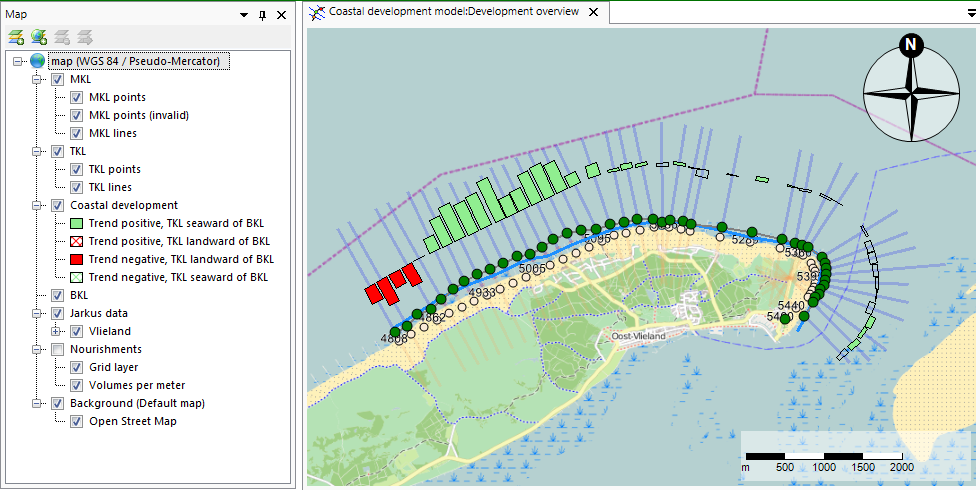
\includegraphics[width=0.85\textwidth]{pictures/Hoofdstuk_Delta_Shell/Map_With_MapContents.png}
		\caption{Voorbeeld van een kaart met resultaten van het Coastal Development Model}
	\label{fig:DS_Map}
\end{figure}

\subsection{Map toolvenster}
	\label{sec:DS_Map_Contents}
Indien een kaart (Map) actief is in het document venster (figuur \ref{fig:DS_Map}), kunnen de kaartlagen worden beheerd in het toolvenster \textbf{Map} (figuur \ref{fig:Map_Contents}).

Met de vier pictogrammen linksboven in het map toolvenster kunnen nieuwe lagen worden toegevoegd of verwijderd op basis van bijvoorbeeld shapefiles (.shp) of TIFF bestanden (.tiff) met georeference. Daarnaast is het mogelijk om een laag op de kaart te exporteren naar een shapefile. Met de knoppen rechtsboven kan het venster worden verwijderd of verborgen. Het venster kan worden opgehaald door te klikken op menu item \textbf{Map} in de \textbf{View} ribbon (zie ook figuur \ref{fig:DS_Ribbon_View}).

Elke laag kan (on)zichtbaar gemaakt worden door het te selecteren of deselecteren. Dit kan gedaan worden voor een laag als geheel, maar ook voor sublagen binnen een laag (indien deze sublagen bevat). Door te dubbelklikken op een laag, wordt de laag properties editor geopend met daarin symbolen, maten, kleuren, etc. Deze eigenschappen kunnen naar voorkeur worden aangepast.

\begin{figure}[h!]
	\centering
		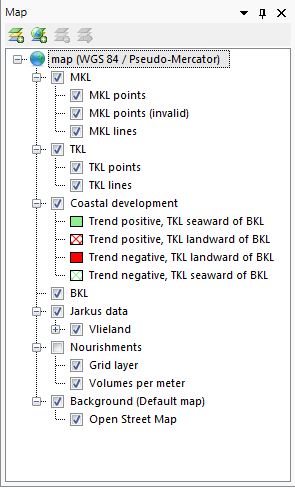
\includegraphics{pictures/Hoofdstuk_Delta_Shell/Map_Contents.png}
		\caption{Voorbeeld van het Map toolvenster waarin verschillende kaartlagen worden getoond. In dit geval gaat het om de kaartlagen van het resultaat van een Momentary coastline model.}
	\label{fig:Map_Contents}
\end{figure}

Door op een laag rechts te klikken wordt een menu geopend dat de mogelijkheden weergeeft voor die laag (figuur \ref{fig:MapLayer_Context_Menu}). Hieronder vallen bijvoorbeeld:
\begin{itemize}
\item \textbf{Properties} - bewerk de styling van de laag. Hiermee kunnen de kleur(schaal) en weergave van de features op deze laag worden aangepast. Tevens is dit de plaats om labels aan of uit te zetten.
\item \textbf{Zoom to Extend} - zet het zoom niveau van de kaart dusdanig dat alle informatie van deze laag precies in het beeld past
\item \textbf{Show in legend} - laat deze laag in de legenda van de kaart zien
\item \textbf{Hide all layers but this one} - laat alleen deze laag op de kaart zien en zet de anderen uit
\end{itemize}

\begin{figure}[h!]
	\centering
		\includegraphics{pictures/Hoofdstuk_Delta_Shell/DS_MapLayer_Context_Menu.png}
		\caption{menu met mogelijkheden na het rechts klikken op een kaartlaag}
	\label{fig:MapLayer_Context_Menu}
\end{figure}

\subsection{Chart toolvenster}
	\label{DS_Chart_Contents}
Indien een document venster een grafiek bevat laat het \textbf{Chart} toolvenster (figuur \ref{fig:3_Chart_Contents}) de afzonderlijk getekende lijnen en punten met hun eigenschappen zien. Door op een item in het toolvenster te klikken (selecteren) wordt in het \textbf{Properties} toolvenster de eigenschappen getoond. Deze kunnen worden bewerkt, zodat bijvoorbeeld het bereik van de assen kan worden veranderd, of kleuren en namen kunnen worden aangepast. Hierdoor is het mogelijk om de figuren met vaste assen te exporteren. Ook kunnen bepaalde lijnen of punten tijdelijk aan of uitgezet worden. In de huidige versie van MorphAn is deze functie helaas nog niet voor de transect editor beschikbaar.

\begin{figure}[H]
	\centering
		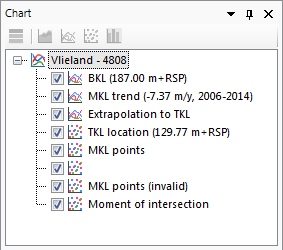
\includegraphics{pictures/Hoofdstuk_Delta_Shell/Chart_Contents.png}
		\caption{Voorbeeld weergave van het Chart toolvenster}
	\label{fig:3_Chart_Contents}
\end{figure}

\subsection{Properties}
Wanneer een element in de interface is geselecteerd (bijvoorbeeld in het project toolvenster of bijvoorbeeld op een kaart, resultaat grafiek of in het chart tool venster) worden de eigenschappen van dit element weergegeven in het properties toolvenster. Naast het geven van een overzicht van de eigenschappen van een geselecteerd element, wordt het properties venster ook gebruikt voor het bewerken van de getoonde eigenschappen.

\subsection{Time Navigator}
	\label{sec:TimeSeriesNavigator}
De time navigator wordt gebruikt om te navigeren door tijd(stappen) van een tijdsafhankelijke variabele. Elk scherm dat tijdsafhankelijke informatie toont heeft zijn eigen time navigator. Hiermee is er de mogelijkheid om te navigeren door de tijd. Deze tijdnavigatie kan twee vormen aannemen:
\begin{itemize}
\item Enkele tijdsindicatie. In dit geval heeft de tijdnavigatie balk een verticale lijn die de positie in de tijd aangeeft. In dit geval wordt slechts een tijdstip weergegeven en wel het tijdstip links van de genoemde lijn (zie figuur \ref{fig:TimeSeriesNavigator}). 
\item Tijd range (figuur \ref{fig:TimeSeriesNavigator_Range}). In dit geval heeft de navigatie balk een rechthoek die begin en eind tijdstip aangeeft. In dit geval worden alle gegevens tussen het begin en eind tijdstip weergegeven.
\end{itemize}

\begin{figure}[H]
	\centering
		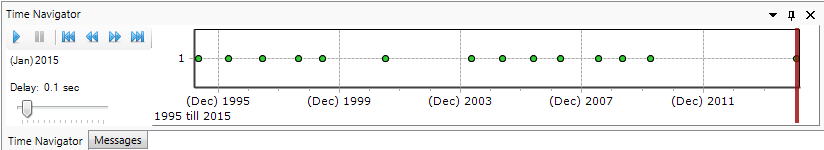
\includegraphics[width=\textwidth]{pictures/Hoofdstuk_Delta_Shell/TimeSeriesNavigator.png}
		\caption{Time Navigator met enkele tijdsindicatie}
	\label{fig:TimeSeriesNavigator}
\end{figure}
\begin{figure}[H]
	\centering
		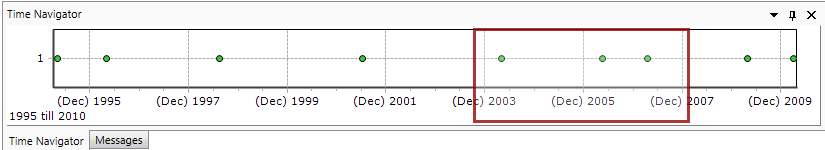
\includegraphics[width=\textwidth]{pictures/Hoofdstuk_Delta_Shell/TimeSeriesNavigator_Range.png}
		\caption{Time Navigator met tijdrange weergave}
	\label{fig:TimeSeriesNavigator_Range}
\end{figure}

\subsection{Messages}
	\label{sec:DS_Messages}
Het message venster is een logging venster. Berichten verstuurd uit modellen of verschillende delen van het systeem worden hier chronologisch getoond. Afhankelijk van de inhoud van het bericht worden deze weergegeven met een icoon (zie voor een verklaring van de iconen tabel \ref{table:message_icons}). Indien het venster wordt gesloten en weer geopend (zie paragraaf \ref{sec:DS_Docking}) worden alleen nieuwe berichten getoond. Oudere berichten worden op twee plaatsen opgeslagen:
\begin{enumerate}
\item Een run rapport wordt getoond in de output folder van het Project toolvenster voor elke modelberekening. Dit run rapport bevat alle berichten die zich voordoen tijdens de berekening.
\item Daarnaast word een applicatie log bijgehouden voor elke sessie (van opstarten tot afsluiten) van MorphAn in de project database. In deze log-file worden alle berichten opgeslagen die zich tijdens de sessie voordoen. De applicatie log kan ten alle tijden worden opgevraagd door in de \textbf{Home} ribbon op de knop \textbf{Show Log} te klikken.
\end{enumerate}

\begin{table}[H]
\caption{Bericht types}
\centering
\begin{tabular}{| c | l |}
\hline
\STRUT{\bf Icoon} & {\bf Bericht type}\\ [1ex]
\hline
\rule{0in}{4ex} 
\includegraphics{pictures/Hoofdstuk_Delta_Shell/Message_Icon_Info.png} & Informatie \\
\hline
\rule{0in}{4ex}

\includegraphics{pictures/Hoofdstuk_Delta_Shell/Message_Icon_Warning.png} & Waarschuwing \\
\hline
\rule{0in}{4ex}

\includegraphics{pictures/Hoofdstuk_Delta_Shell/Message_Icon_Error.png} & Error \\
\hline
\end{tabular}
\label{table:message_icons}
\end{table}

\section {Import \ Export}
Indien voor een item in het \textbf{Project} toolvenster een zogenaamde exporter of importer is gedefinieerd, is het in MorphAn mogelijk om gegevens te exporteren of importeren via het menu onder de rechter muisknop. Kies hiervoor \textbf{Export...} of \textbf{Import...}. Indien een plugin of het framework zelf een exporter of importer voor het geklikte item is aangeboden kan deze worden gebuikt. In sommige gevallen zijn er meerdere manieren om items te exporteren (bijvoorbeeld berekeningsresultaten kunnen als figuur worden ge"exporteerd, maar ook naar het csv format dat in Excel leesbaar is).

MorphAn definieert voor alle berekeningsresultaten een exporter die de resultaten wegschrijft als csv file. Dit format is eenvoudig in Microsoft Excel in te lezen. Let er op dat als scheidingsteken voor de verschillende cellen een "';"' wordt gebruikt en dat in alle gevallen een "'."'  de scheiding tussen gehele getallen en de decimalen aangeeft. Zie ook paragraaf \ref{sec:General_Export_Output}.
\svnid{$Id: ds_overview.tex 1 2015-10-01 14:54:12Z rodriqu_dd $}

\chapter{General overview of the GUI}
\label{chap:ds_overview}

As shown in \Fref{Fig:ArchDS}, one of the interfaces within the framework makes it possible to extend the available (model) plug-ins with Graphical User Interfaces (GUIs). In this fashion, all user interfaces of model plug-ins integrated have the same look-and-feel.

This chapter introduces all GUI-components, which are shared between applications based on the framework.
%
\section{Windows}
\label{sec:windows}
As DeltaShell is an integrated modelling suite, the application is project-based. Within a project several models may be run and combined.

The main user interface is organized in a set of tool and document windows. An example is given in \Fref{fig:fig3.1}. The tool windows show properties of the current project, whereas document windows are used to visualize or edit a specific data type. Tool windows can be docked where you prefer --- even at a second display. Document windows are, when placed within the framework, always in the central area but may also be docked stand-alone (on a second display, for example). Examples of tool windows are:
%
\begin{itemize}
	\item \window{Project}
	\item \window{Map}
	\item \window{Properties}
	\item \window{Chart}
	\item \window{Messages}
\end{itemize}
%
Examples of document windows are:
%
\begin{itemize}
	\item Map(s)
	\item Editor(s)
\end{itemize}
%
\begin{figure} [H]
	\centering
		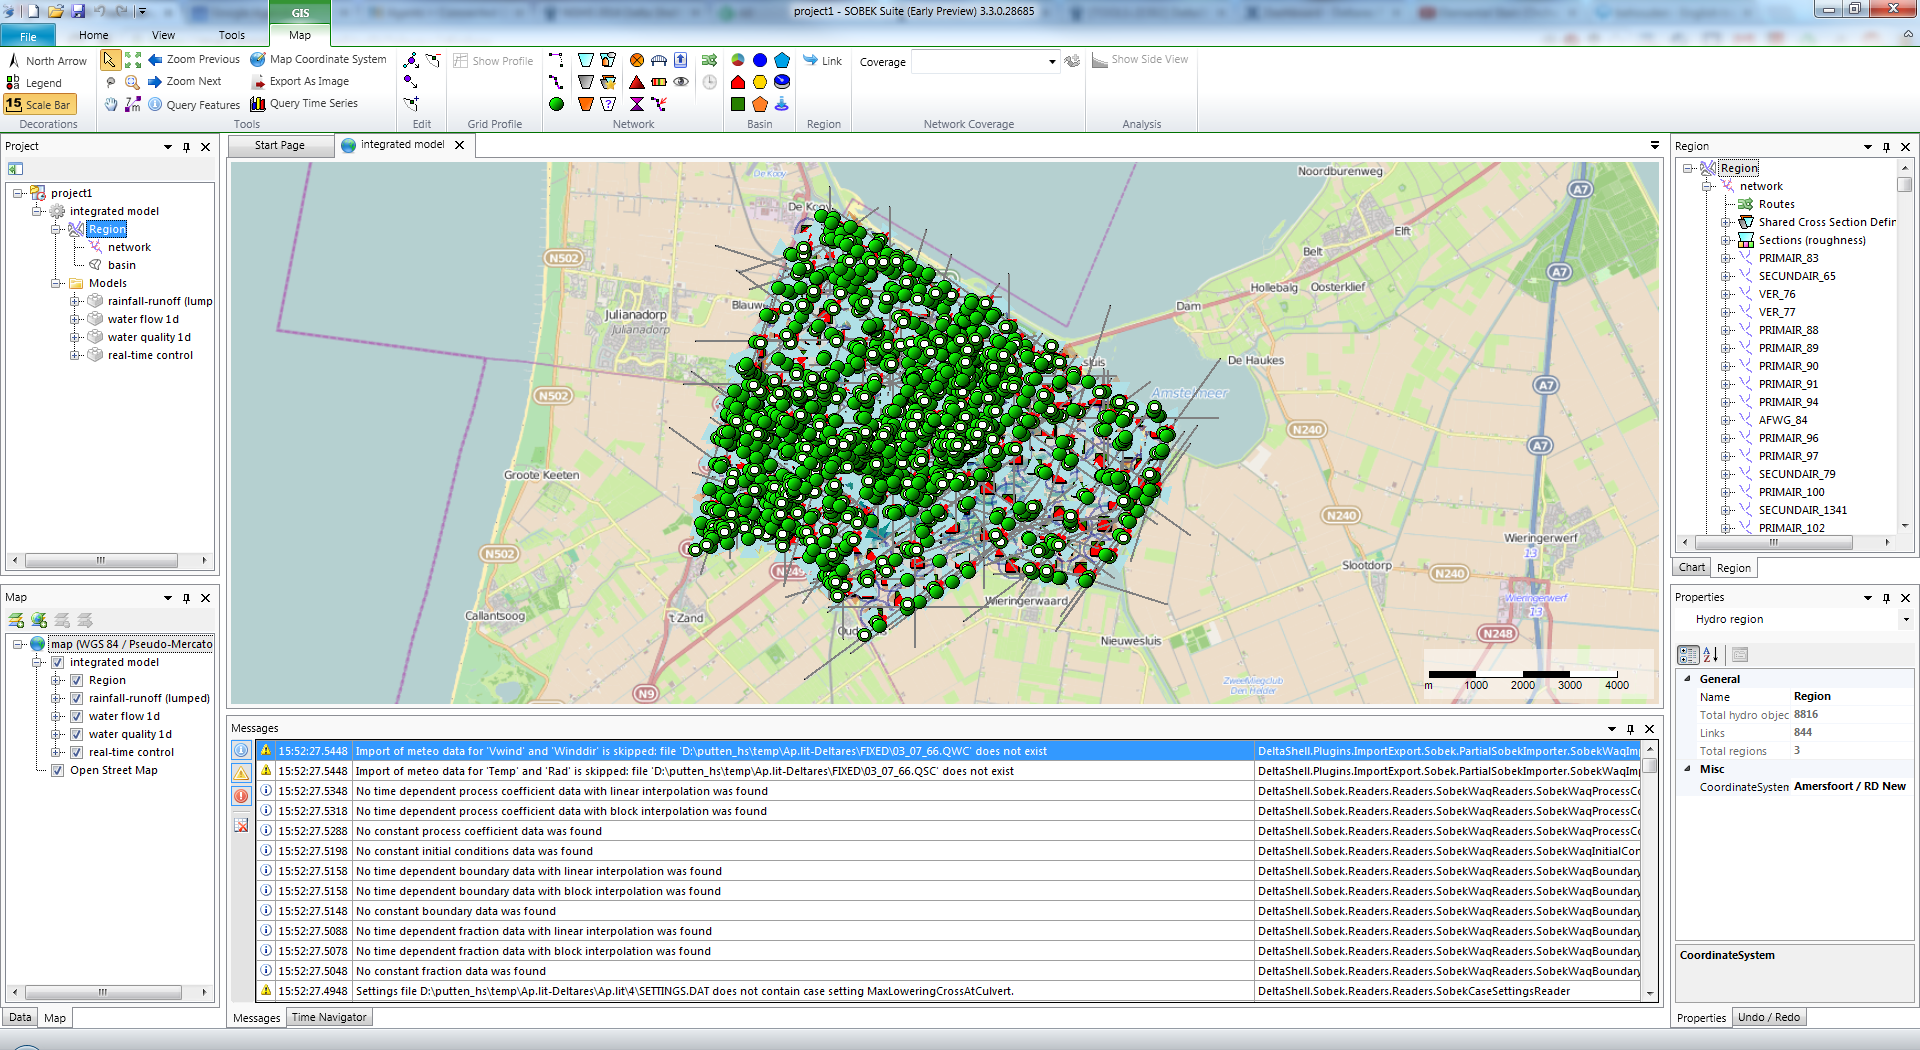
\includegraphics[width=\textwidth]{figures/chapter_overview/overview_ds}
	\caption{Overview of the graphical user interface, example for a SOBEK3 model.}
	\label{fig:fig3.1}
\end{figure}
%
In this chapter all tool windows, menus, dockable views, context menus, and ribbons and toolbars will be described. Map functionality and the spatial editor are treated in separate chapters. The specific editors for the different models are described in the user manuals belonging to those model plug-ins.

\subsection{Project}
\label{subsec:project}
The \window{Project} window is the mainThe \window{Project} window is the main navigation window for the project data, showing the total workspace in a tree view (\Fref{fig:fig2.2}). In the \window{Project} all project components are shown. 
%
All project items with sub-levels can be collapsed by a mouse-click on the `$-$' sign in the tree view. Project data can be sorted by adding new folders to the project tree view and moving models or movable items to designated folders.
%
By clicking on the top left icon in \Fref{fig:fig2.2} the active item in the central Map is located in the tree view.
%
\begin{figure} [H]
	\centering
		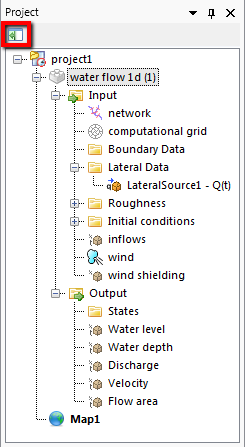
\includegraphics[width=0.5\textwidth]{figures/chapter_overview/view_project_window.png}
	\caption{The project tree window.}
	\label{fig:fig2.2}
\end{figure}
%
Several possibilities exist to work with the tree view:
%
\begin{itemize}
	\item Left mouse-click to select
	\item Right mouse-click gives a context menu with available actions
	\item Double-click to show a map or editor in the main (central) window, depending on the parameter
\end{itemize}
%
\subsection{Main (central) window}
\label{subsec:Main}
The main window (\Fref{fig:fig2.3}) is by default always placed in the middle of the screen. It can also be docked separately, for example on a second display. It is used to present a map for all geo-referenced modeldata, the editors for other data, and results in charts. The editors for other data are model-specific and therefore described in the manuals for the various model plug-ins.

All items with a geo-reference will be presented on the central map, for example: network, computational grid and output data as layers, comparable to a geographical information system (GIS). Working with these layers is described in \Cref{ssec:Map layers}.
%
\begin{figure} [H]
	\centering
		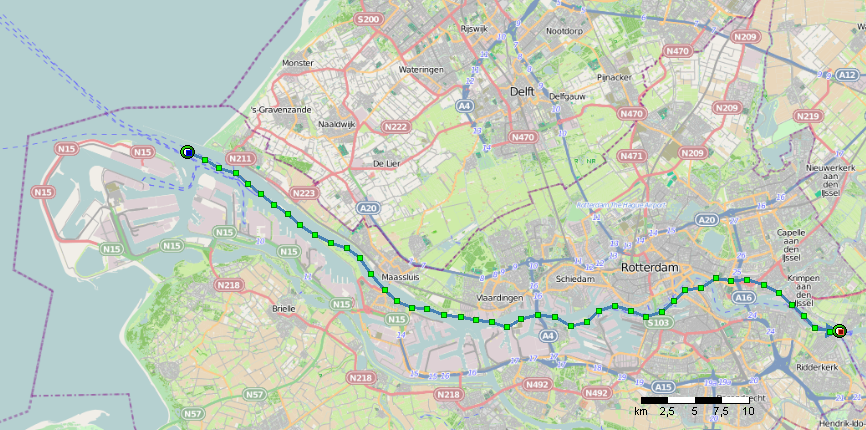
\includegraphics[width=\textwidth]{figures/chapter_overview/example_map.png}
	\caption{The central map view.}
	\label{fig:fig2.3}
\end{figure}
When working in the central map, for example on a network, it is possible to add, adjust or delete network components, which is described thoroughly in the dflow manual.

Results in charts windows (\Fref{fig:chartwindow}) are presented by combining a table view and a '$xy$'-plot. The user can visualize separate data points by selecting rows in the table view. The data that is presented in the chart window may also be exported to a *.csv file by clicking the \button{Csv export} button.
%
\begin{figure} [H]
	\centering
		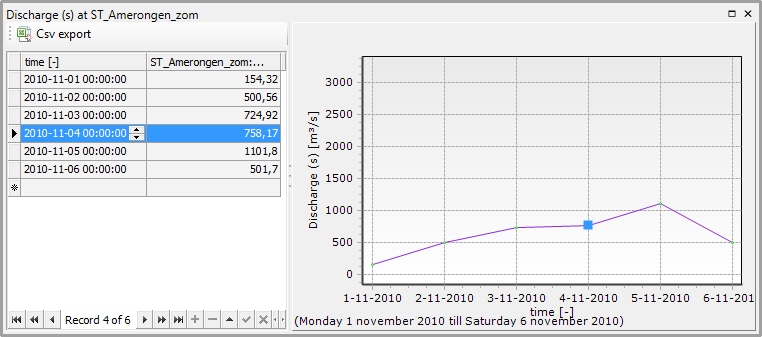
\includegraphics[width=\textwidth]{figures/chapter_overview/example_chart_window.png}
	\caption{The chart window view.}
	\label{fig:chartwindow}
\end{figure}

\subsection{Map}
\label{subsec:Map}
The \window{Map} window (\Fref{fig:fig2.4}) manages the active map. In this window layers within the active map can be shown, hidden or adjusted.
%
With the four icons in the top left of the window new \ext{shp}- or \ext{wms}-layers can be added, removed or exported. With the icons in the top right of the window, the window can be removed or hidden. The window can be retrieved by clicking on \button{Map} in \menu{View} ribbon.
%
\begin{figure} [H]
	\centering
		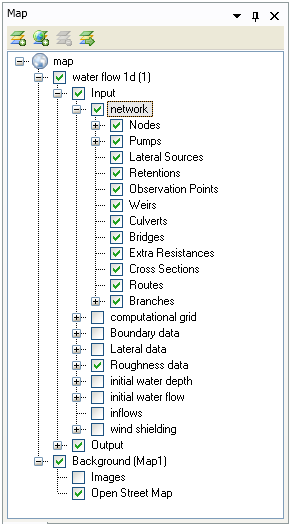
\includegraphics[width=0.5\textwidth]{figures/chapter_overview/view_map_window.png}
	\caption{The map window.}
	\label{fig:fig2.4}
\end{figure}

\subsection{Data}
\label{subsec:data}
The \window{Data} window (\Fref{fig:datawindow}) can be used to inspect the contents of available data items, when selected in the project window.
%
\begin{figure} [H]
	\centering
		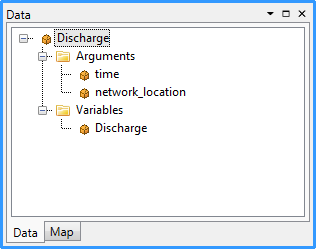
\includegraphics[width=0.5\textwidth]{figures/chapter_overview/view_data_window.png}
	\caption{The data window.}
	\label{fig:datawindow}
\end{figure}

\subsection{Chart}
\label{subsec:chart}
The \window{Chart} window (\Fref{fig:chartwindow}) can be used to stack/unstack chart series of the same type or to convert chart series to a certain type (area, line, point, or bar series), Furthermore, series can be selected or deselected within this window.
 
\begin{figure} [H]
	\centering
		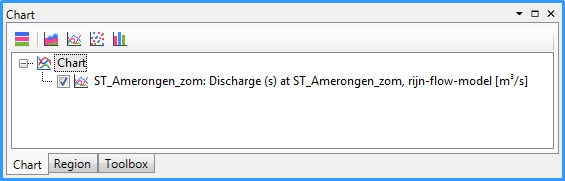
\includegraphics[width=0.5\textwidth]{figures/chapter_overview/view_chart_window.png}
	\caption{Example of the chart window.}
	\label{fig:chartwindow}
\end{figure}
%
\subsection{Properties}
\label{subsec:properties}
%
The \window{Properties} window shows properties for an active selection of the graphical user interface. When a model object is selected in the \window{Region} window it shows the properties of this object. Accordingly, the \window{Properties} window of an item selected in the \window{Project} shows data related to the selected item, for example the simulation time of a \dir{flow model} or a list with output parameters when clicking on the \dir{output} entry. \Fref{fig:fig2.6} shows an example for the properties of a flow model.

In the \window{Properties Window} data can also be edited. If the property grid is insufficient to display the information, for example in case of time series, an additional editor can be opened.
%
\begin{figure} [H]
	\centering
		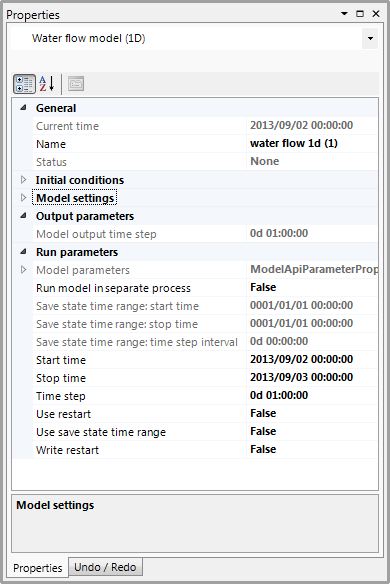
\includegraphics[width=0.5\textwidth]{figures/chapter_overview/view_properties_window.png}
	\caption{Example of a property grid in the properties window of a flow model.}
	\label{fig:fig2.6}
\end{figure}
%
\subsection{Messages}
\label{subsec:messages}
%
The \window{Messages} window (\Fref{fig:messageswindow}) is a logging window. Messages sent from models or different parts of the system are shown here. When a message is too large to fit within the \window{Messages} the user can open a single message (\Fref{fig:messagedetailwindow}) separately by right-mouse-clicking the message and selecting the 'Show details' option.
%
\begin{figure} [H]
	\centering
		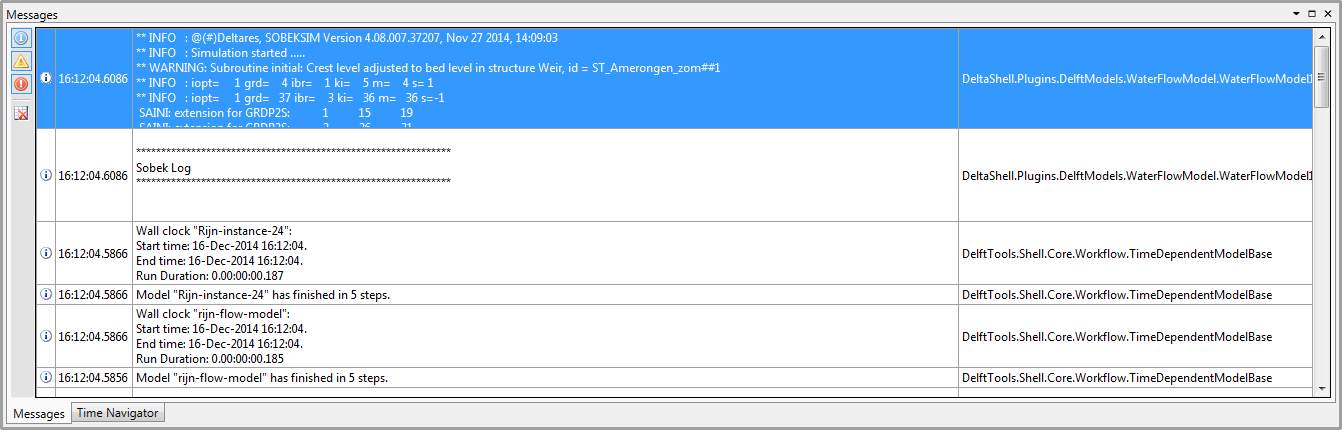
\includegraphics[width=\textwidth]{figures/chapter_overview/view_messages_window.png}
	\caption{The messages window.}
	\label{fig:messageswindow}
\end{figure}
%
\begin{figure} [H]
	\centering
		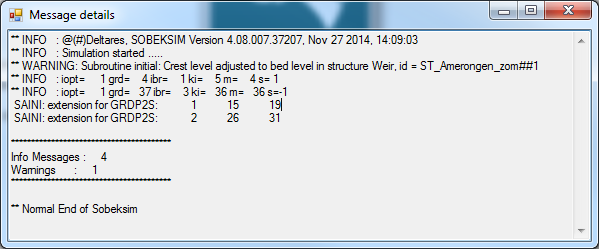
\includegraphics[width=0.5\textwidth]{figures/chapter_overview/view_messagedetails_window.png}
	\caption{The message detail window.}
	\label{fig:messagedetailwindow}
\end{figure} 

Within the \window{Messages} window the user may select the verbosity of the shown messages, ranging from 'Info messages' to 'Warning messages' to 'Error messages'. It is also possible to clear all messages by clicking 
\includegraphics[height=5mm]{figures/chapter_overview/icon_clear_all_messages}.

Furthermore, a run report is shown in the output in the \window{Project} for each model simulation. This run report contains all the messages (from DeltaShell and the model plug-ins) that occur during a simulation.

Finally, an application log is kept for each session of DeltaShell in the project database. In this log-file, which can be accessed through the \menu{File/Help} or \menu{Home} menus, all messages are stored.

% include section: Dockable views, which is also used in other separate User manuals
\svnid{$Id: section_dockableviews.tex 1 2015-08-30 15:39:28Z rodriqu_dd $}

\section{Dockable views}
\label{sec:dockableviews}
The  framework offers lots of freedom to customize dockable views, which are discussed in this section.
\subsection{Docking tabs separately}
\label{subsec:dockingtabs}
Within the  framework the user can dock the separate windows according to personal preferences. These preferences are then saved for future use of the framework. An example of such preferences is presented in \Fref{fig:exampledocking}, where windows have been docked on two screens.
%
\begin{figure} [H]
	\centering
		\includegraphics[width=\textwidth]{figures/chapter_overview/example_docking.png}
	\caption{Docking windows on two screens within the framework.}
	\label{fig:exampledocking}
\end{figure}

\subsection{Multiple tabs}
\label{subsec:multipletabs}
In case two windows are docked in one view, the underlying window (tab) can be brought to the front by simply selecting the tab, as is shown here.
%
\begin{figure} [H]
	\centering
		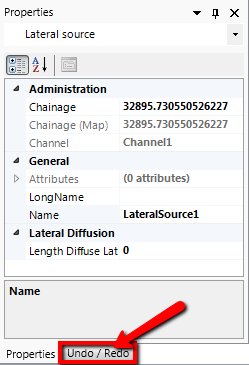
\includegraphics[width=0.5\textwidth]{figures/chapter_overview/example_docking_UndoRedo_1.png}
	\caption{Bringing the \window{Undo/Redo} window to the front}
\end{figure}
%
By dragging dockable windows with the left mouse button and dropping the window left, right, above or below another one the graphical user interface can be customized according to personal preferences. Here an example of the \window{Undo/Redo} window being docked above the \window{Properties} window.
%
\begin{figure} [H]
	\centering
		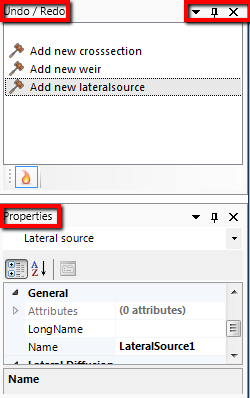
\includegraphics[width=0.5\textwidth]{figures/chapter_overview/example_docking_UndoRedo_2.png}
	\caption{Docking the \window{Undo/Redo} window.}
	\label{fig:docking}
\end{figure}
%
Additional features are the possibility to remove or (auto) hide the window (top right in \Fref{fig:docking}). In case of removal, the window can be retrieved by a mouse-click on \button{Undo/Redo} in the \menu{View} ribbon. Hiding the \window{Undo/Redo} window results in:
%
\begin{figure} [H]
	\centering
		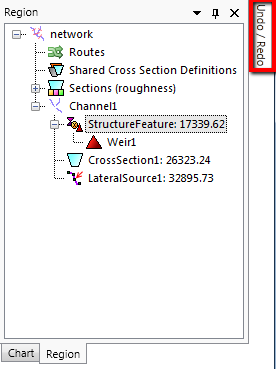
\includegraphics[width=0.5\textwidth]{figures/chapter_overview/example_autohide.png}
	\caption{Auto hide the \window{Undo / Redo} window}
\end{figure}

\section{Context menus}
\label{sec:contextmenus}
Depending on the active window, different context menus are present when right-mouse-clicking on items within this window. This section will treat these context menus per active window. 
%
\subsection{Project}
\label{subsec:project}
Within the \window{Project} window, a variety of levels and/or items with different context menus are present. These will be described here. 
\subsubsection{Project level}
\label{subsubsec:projectlevel}
The context menu of the project level within the project explorer is shown in \Fref{fig:contextmenuproject}. It contains the following choices:
%
\begin{figure} [H]
	\centering
		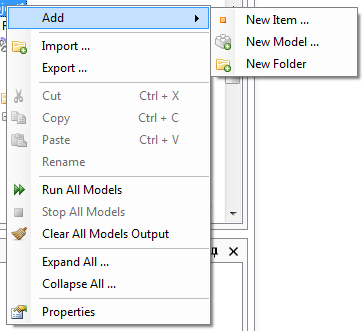
\includegraphics[width=0.5\textwidth]{figures/chapter_overview/context_menu_project.png}
	\caption{The context menu on the project level within the project explorer.}
	\label{fig:contextmenuproject}
\end{figure}
\begin{itemize}
	\item \button{Add} $\Rightarrow$ Option to add models and/or items to project (depending on installed model plug-ins)
	\item \button{Import \dots} $\Rightarrow$ Opens selection window for a variety of available importers (if present)
	\item \button{Export \dots} $\Rightarrow$ Opens selection window for a variety of available exporters (if present) 
	\item \button{Cut} $\Rightarrow$ Cuts current project for pasting elsewhere
	\item \button{Copy} $\Rightarrow$ Copies current project for pasting elsewhere
	\item \button{Paste} $\Rightarrow$ Pastes current project available on the clipboard
	\item \button{Rename} $\Rightarrow$ Rename the current project
	\item \button{Run All Models} $\Rightarrow$ Runs all models available in the project
	\item \button{Stop All Models} $\Rightarrow$ Stops running of all models currently running within the project
	\item \button{Clear All Models Output} $\Rightarrow$ Clears all model output of models available within the project
	\item \button{Expand All \dots} $\Rightarrow$ Expands all project items
	\item \button{Collapse All \dots} $\Rightarrow$ Collapses all project items
	\item \button{Properties} $\Rightarrow$ Switches to \window{Properties} window of active project
\end{itemize}
\subsubsection{Other level still to come}
\label{subsubsec:otherLevel1}
The context menu of \ldots 
%
\subsubsection{Other items}
\label{subsubsec:otheritems}
For the other items in the project explorer the following holds:
\begin{itemize}
	\item Folder items have the same context menu as the project level context menu depicted in \Fref{fig:contextmenuproject}.
	\item All other project items have context menus similar to the context menu on the region level as shown in \Fref{fig:contextmenuregion} 
\end{itemize}

\subsection{Main (Central Map window)}
\label{subsec:centralmap}
The \window{Main} or \window{Central Map} window may consist of multiple tabs \ldots

\subsubsection{Table editor}
\label{subsubsec:tableeditor}
The context menu of the table editors within the \window{Main} window as shown in \Fref{fig:contextmenutable} contains the following choices: 
%
\begin{figure} [H]
	\centering
		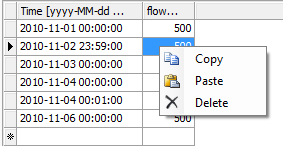
\includegraphics[width=0.4\textwidth]{figures/chapter_overview/context_menu_table.png}
	\caption{The context menu of the table editor.}
	\label{fig:contextmenutable}
\end{figure}
\begin{itemize}
	\item \button{Copy}
	\item \button{Paste}
	\item \button{Delete}
\end{itemize}
\subsubsection{Charts}
\label{subsubsec:charts}
The context menu of the charts within the \window{Main} window as shown in \Fref{fig:contextmenuchart} contains the following choice: 
%
\begin{figure} [H]
	\centering
		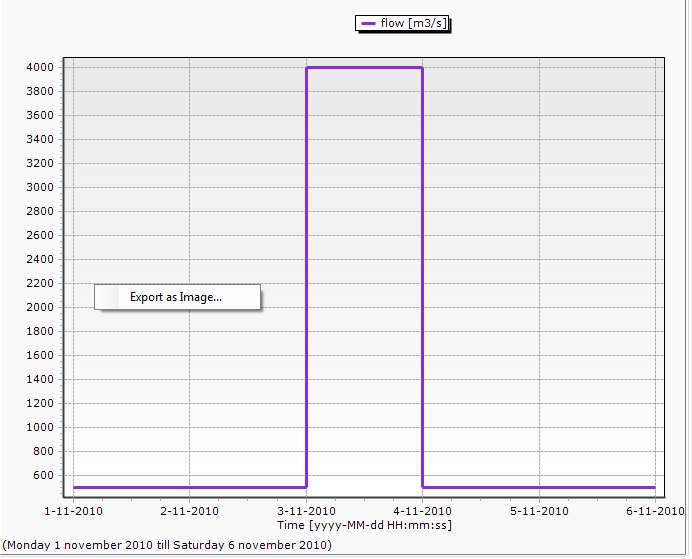
\includegraphics[width=0.8\textwidth]{figures/chapter_overview/context_menu_chart.png}
	\caption{The context menu of the chart view.}
	\label{fig:contextmenuchart}
\end{figure}
\begin{itemize}
	\item \button{Export as Image \dots}
\end{itemize}
\subsection{Map}
\label{subsec:map}
The context menus for the \window{Map} window are described in \Cref{chapter:map}.
%
\subsection{Messages}
\label{subsec:messages2}
The context menu for the \window{Messages} window as shown in \Fref{fig:contextmenumessages} contains the following choices: 
%
\begin{figure} [H]
	\centering
		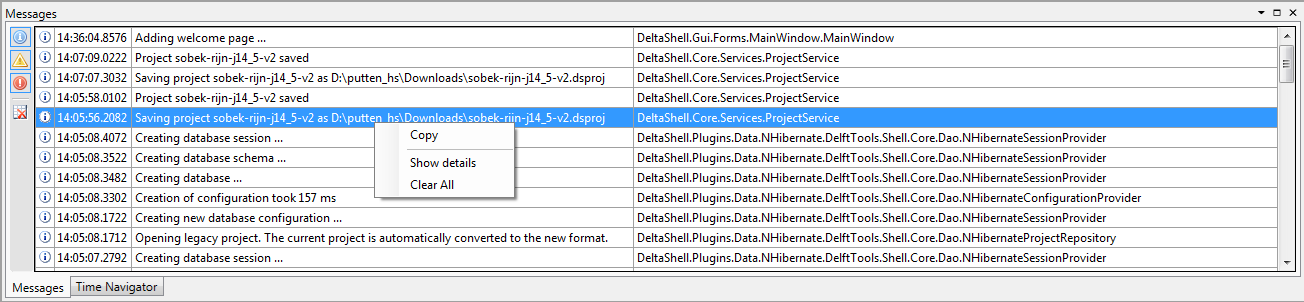
\includegraphics[width=\textwidth]{figures/chapter_overview/context_menu_messages.png}
	\caption{The context menu for the \window{Messages} window.}
	\label{fig:contextmenumessages}
\end{figure}
\begin{itemize}
	\item \button{Copy}
	\item \button{Show details} $\Rightarrow$ Open separate window with detailed message information
	\item \button{Clear all}
\end{itemize}

% include section: Ribbons and toolbars, which is also used in other separate User manuals
\svnid{$Id: section_ribbons.tex 1 2015-08-30 15:39:28Z rodriqu_dd $}

%-------------------------------------------------------------------------------
\section{Ribbons and toolbars}
\label{sec:ribbons}
The user can access the toolbars arranged in \menu{ribbons}. Failure mechanisms plug-ins can have their own specific \menu{ribbon}. The \menu{ribbon} may be auto collapsed by activating the \button{Collapse the Ribbon} button when right-mouse-clicking on the \menu{ribbon}.

%-------------------------------------------------------------------------------
\subsection{Ribbons (hot keys)}\label{subsec:gettingstarted_ribons}

WTI Ringtoets makes use of ribbons, just like Microsoft Office. You can use these ribbons for most of the operations. 
With the ribbons comes hot key functionality, providing shortcuts to perform operations.
If you press ``ALT'', you will see the letters and numbers to access the ribbons and the ribbon contents (i.e.\ operations). For example, ``ALT'' + ``H'' will lead you to the ``Home''-ribbon (\Fref{fig:ribbonhotkey}).

\textbf{\Note Implementation of the hot key functionality is still work in progress.}

\begin{figure}[H]
	\centering
	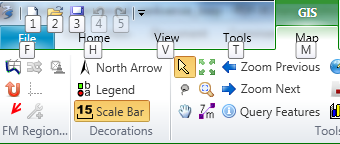
\includegraphics{figures/chapter_overview/ds_ribbon_hotkey.png}
	\caption{Perform operations using the hot keys} \label{fig:ribbonhotkey}
\end{figure}

%-------------------------------------------------------------------------------
\subsection{File}
\label{subsec:file}
The left-most \menu{ribbon} is the \menu{File} ribbon. It has menu-items comparable to most Microsoft applications. Furthermore, it offers users import and export functionality, as well as the \menu{Help} and \menu{Options} dialogs, as shown in \Fref{fig:ribbonfile} and \Fref{fig:dsoptions}.
%
\begin{figure} [H]
	\centering
		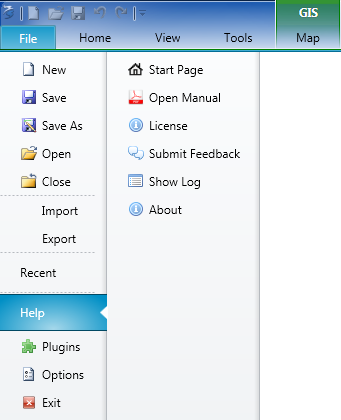
\includegraphics[width=0.6\textwidth]{figures/chapter_overview/ribbon_file.png}
	\caption{The \menu{File} ribbon.}
	\label{fig:ribbonfile}
\end{figure}
%
\begin{figure} [H]
	\centering
		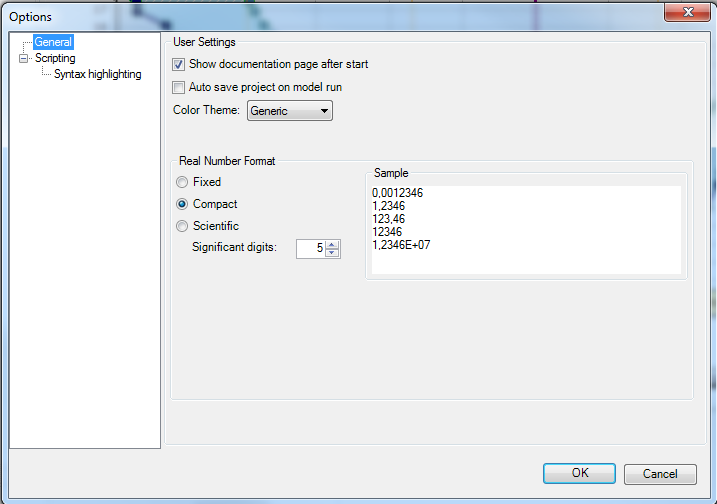
\includegraphics[width=\textwidth]{figures/chapter_overview/ds_options.png}
	\caption{The options dialog.}
	\label{fig:dsoptions}
\end{figure}

%-------------------------------------------------------------------------------
\subsection{Home}
\label{ssec:ribbonhome}
The second \menu{ribbon} is the \menu{Home} ribbon (\Fref{fig:ribbonhome}). It harbours some general features for clipboard actions, addition of items, running models, finding items within projects or views, and help functionality.
\begin{figure}[H]
	\centering
	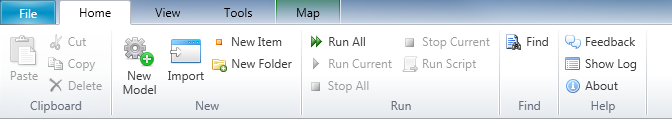
\includegraphics[width=1.0\textwidth]{figures/chapter_overview/ribbon_home.png}
	\caption{The \menu{Home} ribbon.}
	\label{fig:ribbonhome}
\end{figure}
%
%-------------------------------------------------------------------------------
\subsection{View}
\label{ssec:ribbonview}
The third \menu{ribbon} is the \menu{View} ribbon (\Fref{fig:ribbonview}). Here, the user can show or hide windows.
\begin{figure}[H]
	\centering
	\includegraphics[width=0.5\textwidth]{figures/chapter_overview/ribbon_view.png}
	\caption{The \menu{View} ribbon.}
	\label{fig:ribbonview}
\end{figure}
%
%-------------------------------------------------------------------------------
\subsection{Tools}
\label{ssec:ribbontools}
The fourth \menu{ribbon} is the \menu{Tools} ribbon (\Fref{fig:ribbontools}). By default, it contains only the \menu{Open Case Analysis View} tool. Some model plug-ins offer the installation of extra tools that may be installed. These are documented within the user documentation of those model plug-ins. 
\begin{figure}[H]
	\centering
	\includegraphics[width=0.2\textwidth]{figures/chapter_overview/ribbon_tools.png}
	\caption{The \menu{Tools} ribbon.}
	\label{fig:ribbontools}
\end{figure}
%
%-------------------------------------------------------------------------------
\subsection{Map}
\label{ssec:ribbonmap}
The last \menu{ribbon} is the \menu{Map} ribbon (\Fref{fig:ribbonmap}).
\begin{figure}[H]
	\centering
	\includegraphics[width=1.0\textwidth]{figures/chapter_overview/ribbon_map.png}
	\caption{The \menu{Map} ribbon.}
	\label{fig:ribbonmap}
\end{figure}
%
This will be used heavily, while it harbours all \menu{Geospatial} functions, like:
\begin{itemize}
\item \menu{Decorations} for the map
\begin{itemize}
	\item North arrow
	\item Scale bar
	\item Legend
	\item ...
\end{itemize}
\item \menu{Tools} to customize the map view
\begin{itemize}
	\item Select a single item
	\item Select multiple items by drawing a curve
	\item Pan
	\item Zoom to Extents
	\item Zoom by drawing a rectangle
	\item Zoom to Measure distance
	\item ...
\end{itemize}
\item \menu{Edit} polygons, for example within a network, basin, or waterbody
\begin{itemize}
	\item Move geometry point(s)
	\item Add geometry point(s)
	\item Remove geometry point(s)
\end{itemize}
\item Creation of a model \menu{Network}, for example for \dflow
\begin{itemize}
	\item Add new Branch
	\item Split Branch
	\item Add Cross section
	\item Add Weir
	\item Add Pump
	\item ...
\end{itemize}
\end{itemize}
%
\Note The \menu{ribbons} adjust to the size of the application window. If, for what reason, the user wants to minimize the window, the ribbons might look like as shown in \Fref{fig:ribbonmapminimised}. Some of the \menu{ribbon} categories have been condensed into a single drop-down panel.
\begin{figure}[H]
	\centering
	\includegraphics[width=0.8\textwidth]{figures/chapter_overview/ribbon_map_minimised.png}
	\caption{The ribbon with minimized categories.}
	\label{fig:ribbonmapminimised}		
\end{figure}
%
Still, all functions of the category can be activated as they will appear in the drop-down panel.
%
%-------------------------------------------------------------------------------
\subimport{chapters/}{ribbon_scripting}
%
%-------------------------------------------------------------------------------
\subsection{Quick access toolbar}
\label{ssec:Qaccestoolbar}
\Note The user can make frequently used functions available by a single mouse-click in the \menu{Quick Access Toolbar}, the top-most part of the application-window. Do this by right-mouse-clicking a ribbon item and selecting \menu{Add to Quick Access Toolbar}.
%
\begin{figure}[H]
	\centering
	\includegraphics[width=0.6\textwidth]{figures/chapter_overview/quick_access_toolbar.png}
	\caption{The quick access toolbar.}
	\label{fig:qat}		
\end{figure}

%\appendix
%\svnid{$Id: A_How_to_use_OpenDA_models.tex 1 2015-10-01 15:39:28Z rodriqu_dd $}

\chapter{Example of an appendix}\label{How_to_use_OpenDA_models}

%include text from common, as this is shared with the Delta Shell User Manual
\svnid{$Id: Appendix1_text.tex 1 2015-08-30 15:39:28Z rodriqu_dd $}

%this text can be shared between several User Manuals

\section{Introduction} \label{sec:Appendix1Intro}

Here goes the introduction to this appendix. 
\section{Second section of this appendix} \label{sec:Appendix1Section2}

\subsection{Subsection in second section of this appendix}

Blah, blah, blah,...


\subsection{And another subsection}

With more text in here.

\section{Last section}

The text of the last section.



\cleardoublepage
%
\newpage
\pagestyle{empty}
\mbox{}
\includepdf[pages=2,offset=-72 -70]{cover/default-cover-pages.pdf} % links-rechts past precies
\end{document}